\begin{problem}{청소}
	{standard input}{standard output}
	{18 seconds}{2048 megabytes}{}
	
	비타로의 방은 밑변의 길이가 $N$인 직각이등변삼각형 모양이다. 비타로의 방의 위치는 $0 \le x \le N$, $0 \le y \le N$, $x+y \le N$을 만족하는 $(x, y)$로 표현된다. 직각인 꼭짓점이 원점이다. 두 밑변은 $x$축과 $y$축이다.
	
	\begin{center}
		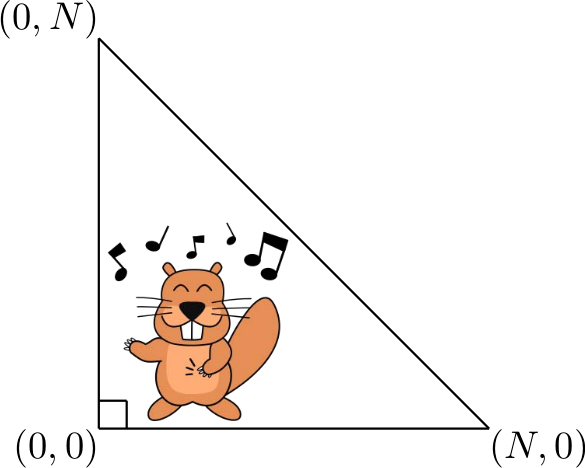
\includegraphics[width=0.5\linewidth]{img1.png}
	\end{center}
	
	
	
	어느 날, 비타로는 방이 먼지로 가득 찬 것을 발견했다. 처음에 방에는 $M$개의 먼지가 있다. $i$번 ($1 \le i \le M$) 먼지는 $(X_i, Y_i)$에 놓여 있다. 둘 이상의 먼지가 같은 곳에 있을 수도 있다.
	
	이제, 비타로는 빗자루를 이용하여 집을 청소하려고 한다. 우리는 빗자루를 방 안에 있는 선분이라고 생각한다. 이 선분의 길이를 \textbf{너비}라고 한다. 비타로는 다음 두 방법으로만 빗자루질한다.
	
	
	\begin{itemize}
		\item 비타로는 빗자루를 한 점을 원점에 놓고 $y$축과 평행하게 놓는다. 그리고 빗자루를 $x$축 양의 방향으로 움직이면서 빗자루의 한 점이 $x$축 위에 있고 $y$축과 평행하도록 움직일 수 있을 때까지 움직인다. 빗자루의 너비가 $l$이라면, $x<N-l$과 $y \le l$을 만족하는 $(x, y)$에 있는 먼지는 $(N-l, y)$로 움직일 것이다. ($(N-l, y)$에 다른 먼지가 있을 수도 있다.) 이 방법을 \textbf{H 쓸기} 라고 한다.
		
		\item 비타로는 빗자루를 한 점을 원점에 놓고 $x$축과 평행하게 놓는다. 그리고 빗자루를 $y$축 양의 방향으로 움직이면서 빗자루의 한 점이 $y$축 위에 있고 $x$축과 평행하도록 움직일 수 있을 때까지 움직인다. 빗자루의 너비가 $l$이라면, $x\le l$과 $y < N-l$을 만족하는 $(x, y)$에 있는 먼지는 $(x, N-l)$로 움직일 것이다. ($(x, N-l)$에 다른 먼지가 있을 수도 있다.) 이 방법을 \textbf{V 쓸기} 라고 한다.
	\end{itemize}
	
	비타로의 방에서 $Q$개의 일이 차례로 일어날 것이다. $j$ 번째 ($1 \le j \le Q$) 일은 다음 중 하나이다.
	
	\begin{itemize}
		\item $P_j$ 번째 먼지의 좌표를 계산한다.
		\item 너비 $L_j$인 빗자루를 사용하여, H 쓸기를 한다.
		\item 너비 $L_j$인 빗자루를 사용하여, V 쓸기를 한다.
		\item $(A_j, B_j)$에 새로운 먼지가 추가된다. 이 일 전에 $c$ 개의 먼지가 있었다면, 이 먼지는 $(c+1)$ 번째 먼지이다.
	\end{itemize}
	
	방의 밑변의 길이, 방에 있는 먼지의 좌표와 일어난 일들이 주어졌을 때, 먼지의 좌표를 계산하여라.
	
	\InputFile
	
	표준 입력에서 다음과 같은 형식으로 주어진다. 모든 수는 정수이다.
	
	$N$ $M$ $Q$
	
	$X_1$ $Y_1$
	
	$\vdots$
	
	$X_M$ $Y_M$ 
	
	(Query 1)
	
	$\vdots$
	
	(Query Q)
	
	공백으로 구분 된 두 개 혹은 세 개의 수가 (Query $j$) ($1 \le j \le Q$) 로 주어진다. $T_j$가 첫 번째 수라고 하자. 이 줄의 의미는 다음과 같다.
	
	\begin{itemize}
		\item $T_j=1$이면, 두 정수 $T_j$, $P_j$가 공백으로 구분되어 주어진다. 이는 $j$ 번째 일이 비타로가 $P_j$의 위치를 계산하는 것을 의미한다.
		\item $T_j=2$이면, 두 정수 $T_j$, $L_j$가 공백으로 구분되어 주어진다. 이는 $j$ 번째 일이 비타로가 너비 $L_j$인 빗자루를 사용하여 H 쓸기를 하는 것을 의미한다.
		\item $T_j=3$이면, 두 정수 $T_j$, $L_j$가 공백으로 구분되어 주어진다. 이는 $j$ 번째 일이 비타로가 너비 $L_j$인 빗자루를 사용하여 V 쓸기를 하는 것을 의미한다.
		\item $T_j=4$이면, 세 정수 $T_j$, $A_j$, $B_j$가 공백으로 구분되어 주어진다. 이는 $j$ 번째 일이 새 먼지가 $(A_j, B_j)$에 추가 된 것을 의미한다.
	\end{itemize}
	
	
	\OutputFile
	
	
	$T_j=1$인 일이 생길 때마다, 하나의 줄을 표준 출력으로 출력하여라. $j$ 번째 일이 생길 때에 $P_j$의 $x$좌표와 $y$좌표를 공백으로 구분하여 출력하여라.
	
	

	\Constraints


	\begin{itemize}
		
		\item $1 \le N \le 1\ 000\ 000\ 000$.
		\item $1 \le M \le 500\ 000$.
		\item $1 \le Q \le 1\ 000\ 000$.
		\item $0 \le X_i \le N$ ($1 \le i \le M$).
		\item $0 \le Y_i \le N$ ($1 \le i \le M$).
		\item $X_i + Y+i \le N$ ($1 \le i \le M$).
		\item $1 \le P_j \le (j$ 번째 일이 생길 때 먼지 개수$)$ ($1 \le j \le Q$).
		\item $0 \le L_j \le N-1$ ($1 \le j \le Q$).
		\item $0 \le A_j \le N$ ($1 \le j \le Q$).
		\item $0 \le B_j \le N$ ($1 \le j \le Q$).
		\item $A_j + B_j \le N$ ($1 \le j \le Q$).
		\item $T_j = 1$인 일이 적어도 하나 존재한다. ($1 \le j \le Q$).
	\end{itemize}


	\SubtaskWithCost{1}{1}
	\begin{itemize}
		\item $M \le 2\ 000$.
		\item $Q \le 5\ 000$.
	\end{itemize}

	
	\SubtaskWithCost{2}{10}
	\begin{itemize}
		\item $T_j = 1, 2, 4$.
	\end{itemize}


	\SubtaskWithCost{3}{11}
	\begin{itemize}
		\item $T_j = 1, 2, 3$.
		\item $X_j \le X_{j+1}$ ($1 \le j \le M-1$).
		\item $Y_j \ge Y_{j+1}$ ($1 \le j \le M-1$).
	\end{itemize}

	
	\SubtaskWithCost{4}{53}
	\begin{itemize}
		\item $T_j = 1, 2, 3$.
	\end{itemize}
	
	\SubtaskWithCost{5}{25}
	
	추가 제한조건이 없다.
		
	\Examples
		
	\begin{example}
	\exmp{
6 2 10
1 1
4 0
4 2 3
3 3 
1 1
4 1 2
2 3
2 0
1 4
3 2 
1 3
1 2
	}{%
1 3
3 2
3 3
6 0
	}%
\end{example}

	\begin{itemize}
		\item 처음에 첫 번째 먼지가 $(1, 1)$, 두 번째 먼지가 $(4, 0)$에 있다. (그림 1)이 방의 상태이다.
		\item 첫 번째 일에서 세 번째 먼지가 $(2, 3)$에 놓인다. (그림 2)가 방의 상태이다.
		\item 두 번째 일에서 너비 3의 빗자루로 V 쓸기를 한다. 그 후, 첫 번째 먼지가 $(1, 3)$ 으로 옮겨졌다. (그림 3)이 방의 상태이다.
		\item 세 번째 일에서 첫 번째 먼지의 좌표인 $(1, 3)$을 계산한다.
		\item 네 번째 일에서 네 번째 먼지가 $(1, 2)$에 놓인다. (그림 4)가 방의 상태이다.
		\item 다섯 번째 일에서 너비 3의 빗자루로 H 쓸기를 한다. 그 후, 첫 번째 먼지가 $(3, 3)$ 으로, 세 번째 먼지가 $(3, 3)$으로, 네 번째 먼지가 $(3, 2)$로 옮겨졌다. (그림 5)가 방의 상태이다.
		\item 여섯 번째 일에서, 너비 0의 빗자루로 H 쓸기를 한다. 그 후, 두 번째 먼지가 $(6, 0)$ 으로 옮겨졌다. (그림 6)이 방의 상태이다.
		\item 일곱 번째 일에서, 비타로는 네 번째 먼지의 좌표인 $(3, 2)$를 계산한다.
		\item 여덟 번째 일에서, 비타로는 너비 2의 빗자루로 V 쓸기를 한다. 어떤 먼지도 옮겨지지 않았다. (그림 7)이 방의 상태이다.
		\item 아홉 번째 일에서, 비타로는 세 번째 먼지의 좌표인 $(3, 3)$을 계산한다.
		\item 열 번째 일에서, 비타로는 두 번째 먼지의 좌표인 $(6, 0)$을 계산한다.
	\end{itemize}

	이 예제는 서브태스크 1과 5의 조건을 만족한다.

	\begin{center}
	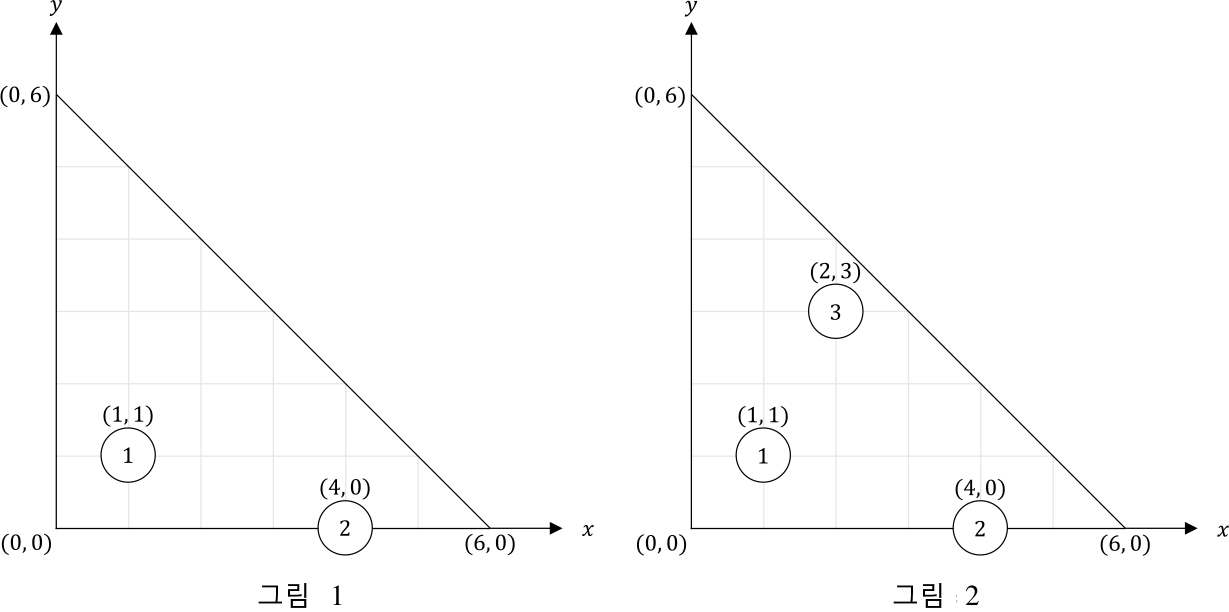
\includegraphics[width=\linewidth]{img2.png}
	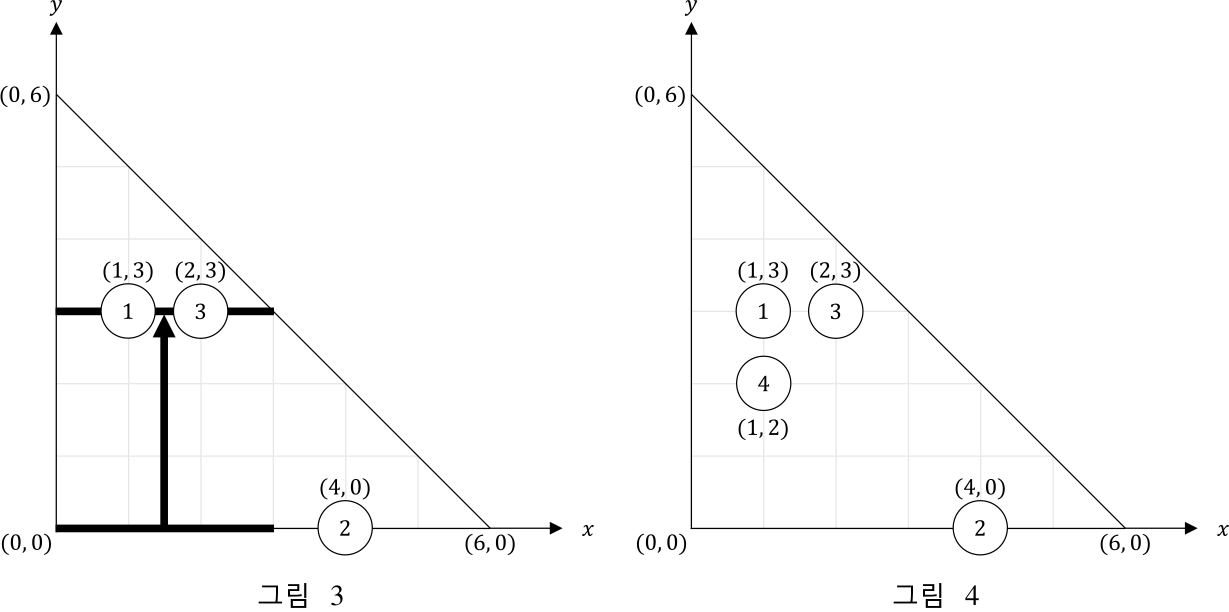
\includegraphics[width=\linewidth]{img3.png}
	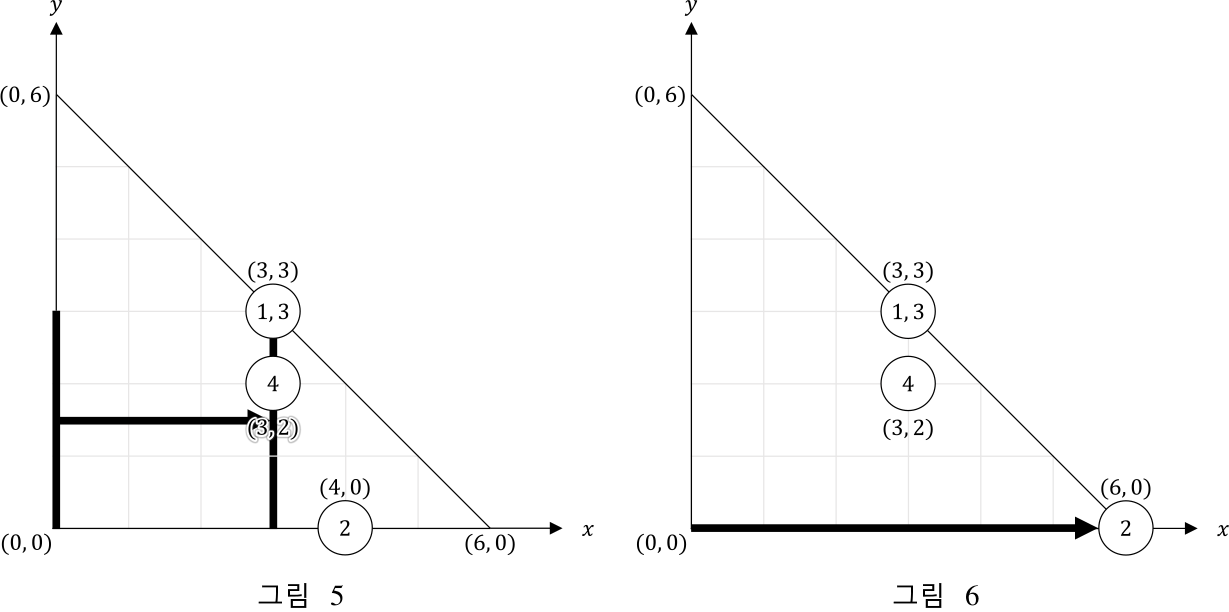
\includegraphics[width=\linewidth]{img4.png}
	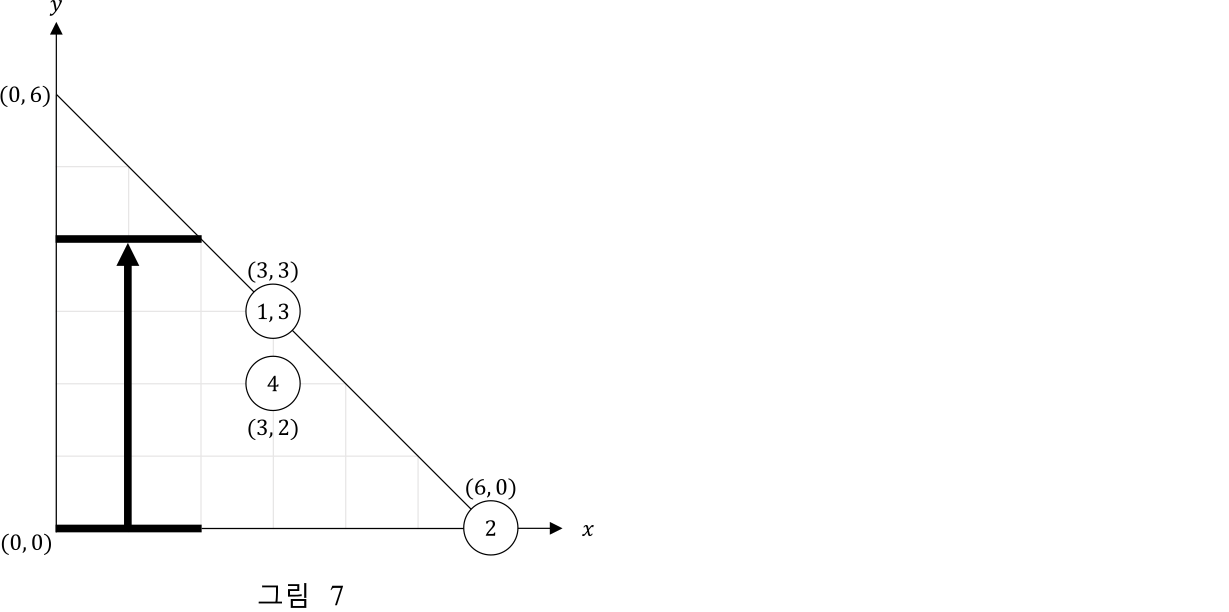
\includegraphics[width=\linewidth]{img5.png}
	\end{center}


	\begin{example}
	\exmp{
		9 4 8
		2 3
		3 1
		1 6
		4 3
		2 6
		1 3
		2 2
		1 4
		2 3
		1 2
		2 4
		1 1
	}{%
		3 6
		4 3
		7 1
		6 3
	}%
	\end{example}

	이 예제는 서브태스크 1, 2, 4와 5의 조건을 만족한다.
	

	\begin{example}
	\exmp{
		8 1 8
		1 5
		4 4 1
		2 6
		1 2
		2 3
		4 2 2
		2 5
		1 1
		1 3
	}{%
		4 1
		3 5
		3 2
	}%
	\end{example}

	이 예제는 서브태스크 1, 2와 5의 조건을 만족한다.


	\begin{example}
		\exmp{
			7 4 9
			1 5
			2 2
			4 2
			5 0
			2 6
			2 3
			1 2
			3 6
			1 4
			3 1
			1 1
			2 2
			1 3
		}{%
			4 2
			5 1
			1 6
			5 2
		}%
	\end{example}
	
	이 예제는 서브태스크 1, 3, 4와 5의 조건을 만족한다.

	
\end{problem}

